\subsection{Specular lighting}
The specular lighting element uses the angles between a surface's normal
$\vec{N}$ and the direction to the light source $\vec{l}$, and to the point of
view $\vec{V}$ respectively, to determine an intensity weight based the amount
of light reflected in the direction of the viewer. Intuitively, the result
should be inversely proportional to $\alpha$. See figure \ref{fig:specAng}

The specular element is found by
$$I_{specular} = I_{s}K_{s}(\vec{R}\cdot\vec{V})^e$$
where $\vec{R}$ is $\vec{l}$ mirrored around $\vec{N}$, and $e$ is a measure of
the specularity sharpness.

\begin{figure}[!hbtp]
	\centering
	\scalebox{0.7}
	{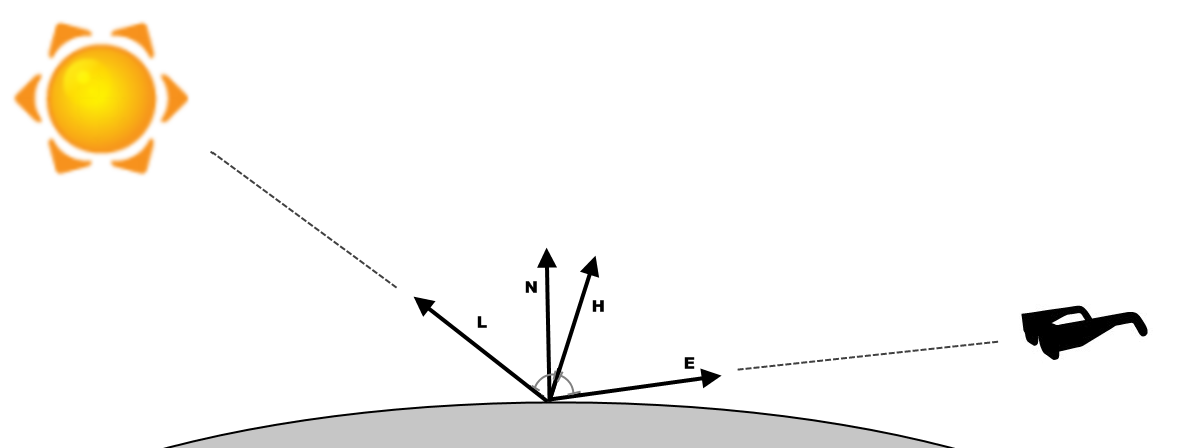
\includegraphics{pics/specularAngle.png}}
	\caption{}
	\label{fig:specAng}
\end{figure}
